% !TEX root = ../main.tex

\chapter{散射尾波}

\section{超声波在颗粒介质中的扩散近似}

\subsection{理论推导}

波在强散射介质中的传播是一个古老的问题。Weaver R. L. 根据 RTE 推导出了超声波脉冲在多晶体中的扩散行为方程\cite{diffusivity}:

\begin{equation}
  \frac{\partial I}{\partial t} - D\nabla^{2}I + \frac{I}{\tau_{\alpha}} = \delta(z)\delta(t)
\end{equation}

其中 $D$ 是扩散系数,$\tau_{\alpha}$ 是描述信号强度在时域上衰减行为的特征时间,$z$ 是圆柱坐标系中的轴向坐标。因为是超声波脉冲(中心频率充分大、脉冲宽度充分小),即视为时域和空间上的 Dirac 函数 $\delta{z}\delta(t)$。

因为在实际的实验中,我们使用的颗粒容器是圆筒形,所以在求解强度方程时可以采用圆柱对称处理;又因为亚克力板容器壁厚达 10 \unit{\milli\meter} 而假定容器边界的声阻抗足够大,在这种情形下声信号在容器壁全反射。在以上条件下,得出的进入底部探头的透射通量\cite{PhysRevLett.93.154303}为

\begin{equation}
  J(t) = \frac{\nu_{e} U_{0}}{2L}{\ee}^{-\frac{t}{\tau_{\alpha}}}\sum_{n=0}^{\infty}\frac{(-1)^{n}}{\delta_{n}}\cos{\left(\frac{n\uppi l^{*}}{L}\right)}{\ee}^{-\frac{D(n\uppi)^{2}t}{L^{2}}},\quad \delta_{n} = \begin{cases}
    2, & n = 0, \\
    1, & \text{otherwise}.
  \end{cases}
\end{equation}

其中 $U_{0}$ 是声源能量, $D = \frac{1}{3}\nu_{e}l^{*}$ 为扩散系数, $\nu_{e}$ 为能量传输速度, $l^{*}$ 为平均自由程, $\tau_{\alpha}$ 正式名为非弹性吸收时间。在实验中,我们用飞行时间法测定的声速 $V_{\text{T.O.F.}}$ 来替代 $\nu_{e}$。质量因子 $Q = 2\pi f\tau_{\alpha}$ 也被引入用于描述颗粒介质的耗散性,其中 $f$ 是发射信号的中心频率。Jia 提出了在颗粒表面相对平滑时,存在关系\cite{PhysRevLett.101.138001}

\begin{equation}
  Q^{-1} = \left[\frac{4G_{g}}{9\uppi^2(2-\nu_{g})R}\left(\frac{3\uppi}{4K_{g}}\right)^{\frac{1}{3}}\right]\mu^{-1}P_{0}^{-\frac{2}{3}}u_{t}
\end{equation}

其中 $\nu_{g}$、$K_{g}$、$G_{g}$ 是颗粒组成材料的泊松比、体弹性模量和剪切模量,$R$ 是颗粒半径,$\mu$ 用于描述颗粒间的摩擦系数,$P_{0}$ 是颗粒介质所受的应力大小,$u_{t}$ 是描述 Mindlin 接触的切向振幅。在受到润滑作用的时候,还存在 $Q^{-1} = Q_{\text{fric}}^{-1} + Q_{\text{vis}}^{-1}$ 的修正关系,在这里由于在实验中未涉及而不再额外讨论。

对于摩擦系数 $\mu$ 的理解,需要将其和后文中的式~\eqref{eq:friction} 中的摩擦系数配合理解。经验丰富的工人观察沙堆的半径或者高度即可估算沙堆的体积,原理就是因为沙堆是通过类似于点源法/有限面元法的方式制备的,其斜坡角度/休止角(repose angle)通常固定;这里的角度通常都是\numrange{0}{45} \unit{\degree} 范围内的,对应于其正切值的摩擦系数范围是 \numrange{0}{1})。这与上式中的有时大于 1 的 $\mu$ 显然并不相同。

\subsection{实验验证}



\section{超声波在颗粒介质中的非线性}

%\subsection{线性响应理论}
% 老师声称这个可以用来水字数,但是是这样吗?

\subsection{非线性波方程与各级谐波}

在连续介质力学中,我们已经学习过描述声波传播的 Burgers 方程:

\begin{align}
  \frac{\partial p}{\partial x} - \frac{\delta}{2c_{0}^{3}}\frac{\partial^{2}p}{\partial t^{2}} = \frac{\beta p}{\rho_{0}c_{0}^{3}}\frac{\partial p}{\partial t},\label{eq:burgers_equation_1}\\
  \delta = \frac{1}{\rho_{0}}\left[\frac{4}{3}\mu + \mu_{B} + \kappa\left(\frac{1}{c_{v}} - \frac{1}{c_{p}}\right)\right].
\end{align}

其中 $\mu$ 是介质的剪切黏度,$\mu_{B}$ 是介质的容变黏度,这两者共同构成了介质的黏性吸收;$\kappa$ 是介质的热导率,$c_{v}$ 是介质的定容热容,$c_{p}$ 是介质的定压热容,这两者构成了介质的热传导吸收。两者的线性叠加构成了 Stokes-Kirchhoff 衰减公式,用于描述声波在介质中传播时的经典吸收现象。$\beta$ 是介质的非线性系数,$\rho_{0}$ 和 $c_{0}$ 分别是介质在平衡态下的密度和声速。

Mendousse 首个推导出专用于平面波声传播的偏微分方程。他设定具有黏度的理想气体,根据 Navior-Stockes 方程写出一维流动形式的 Lagrangian 量\cite{hamilton_nonlinear_1998}:

\begin{equation}
  \rho_{0}\frac{\partial^{2}\xi}{\partial t^{2}} - \frac{4}{3}\mu\frac{\partial }{\partial a}\left[\left(1 + \frac{\partial\xi}{\partial a}\right)\frac{\partial^{2}\xi}{\partial a\partial t}\right] + \frac{\partial P}{\partial a} = 0.\label{eq:mendousse_equation}
\end{equation}

其中,$\xi$ 是参考于物质位置 $a$ 的流体粒子位移量,即存在坐标关系为

\begin{equation}
  x = a + \xi(a,t).
\end{equation}

Mendousse 假定黏性吸收中由体变黏度 $\mu_{B}$ 和热导率 $\kappa$ 引起的吸收远小于由剪切黏度 $\mu$ 所引起的从而只保留了后者,并且在黏性项中忽略了本应存在的系数 $1+\partial\xi/\partial a$。考虑到流体中局域的质量守恒规则,我们可以得到平衡态下的密度和流变密度之间的关系:

\begin{equation}
  \rho_{0} = \left(1 + \frac{\partial\xi}{\partial a}\right)\rho,
\end{equation}

由于忽略了黏度相关的一个二阶项,总压力 $P$ 对 $\partial\xi/\partial a$ 的级数展开化为

\begin{equation}
  P = P_{0} - \rho_{0}c_{0}^{2}\left[\frac{\partial\xi}{\partial a} - \beta\left(\frac{\partial\xi}{\partial a}\right)^{2}\right],
\end{equation}

所以式~\eqref{eq:mendousse_equation} 化为下式:

\begin{equation}
  \rho_{0}\frac{\partial^{2}\xi}{\partial t^{2}} - \rho_{0}\delta\frac{\partial^{3}\xi}{\partial a^{2}\partial t} - \rho_{0}c_{0}^{2}\frac{\partial^{2}\xi}{\partial a^{2}} + 2\rho_{0}c_{0}^{2}\beta\frac{\partial\xi}{\partial a}\frac{\partial^{2}\xi}{\partial a^{2}} = 0,\label{eq:progressive_burgers_equation}
\end{equation}

对于角频率为 $\omega$ 的正弦波在诸如上述方程所控制下的传播,其产生的畸变与失真可以理解为产生高次谐波的过程。因此通过级数展开求解式~\eqref{eq:progressive_burgers_equation},依次得到基波、各级谐波的表达式:

\begin{equation}
  \begin{cases}
    u_{1\omega}(a,t) &\approx u_{\text{in}}e^{-a\alpha}\cos{(ka-\omega t)}\\
    u_{2\omega}(a,t) &\approx \frac{u_{\text{in}}^{2}}{8}\left(\frac{\beta\omega^{2}}{\alpha c_{0}^{2}}\right)e^{-2\alpha a}\cos{[2(ka-\omega t)]}\\
    u_{3\omega}(a,t) &\approx \frac{u_{\text{in}}^{3}}{48}\left(\frac{\beta\omega^{2}}{\alpha c_{0}^{2}}\right)^{2}e^{-3\alpha a}\cos{[3(ka-\omega t)]}
    \end{cases}
\end{equation}

其中 $u_{\text{in}}$ 是声源振幅,$a$ 是声波传播距离,$\alpha$ 是声波的衰减系数,$k$ 是声波的波数,$\omega$ 是声波的频率。$u_{n\omega}$ 代表 $n$ 倍频的谐波振幅($n=1$ 即为基波)。我们很容易以一个简单的公式总结各谐波振幅与源振幅的关系:

\begin{equation}
  u_{n\omega} \propto \left(u_{\text{in}}\right)^{n}.\label{eq:harmonic_linear}
\end{equation}

颗粒介质具有强耗散性,我们可以将这种信号在颗粒介质中的衰减类比于声波在具有切变黏性 $\mu$ 的流体中传播时所受的黏性吸收作用,即使用等效黏度 $\mu^{*}$ 来对颗粒介质进行宏观的统计性描述。如果式~\eqref{eq:harmonic_linear} 描述的线性关系随着声源振幅 $u_{\text{in}}$ 增大遭到破坏,即说明等效黏度已经因为泵浦作用发生变化。对于水和空气这类连续介质,在黏性力相较于弹性力很小时,存在描述衰减 $\alpha$ 与声波角频率 $\omega$ 的指数关系:

\begin{equation}
  \alpha = \alpha_{\mu} + \alpha_{h} = \frac{\omega^{2}}{2\rho_{0}c_{0}^{3}}\left[\frac{4}{3}\mu + \mu_{B} + \kappa\left(\frac{1}{c_{v}} - \frac{1}{c_{p}}\right)\right]\propto \omega^{2}
\end{equation}

其中 $\alpha_{\mu}$ 和 $\alpha_{h}$ 分别是描述黏性吸收和热传导吸收的衰减系数。在后文中我们将组织实验来验证通过接触力相联系的颗粒介质中,是否同样存在着类似的衰减系数 $\alpha^{*}$ 与信号角频率 $\omega$ 之间的指数关系。

\subsection{相似性参数}

引入交叉关联函数(cross-relation function)作为相似性参数 $\Psi_{i,j}(\tau)$, 以描述信号 $S_{i}$ 与 $S_{j}$ 的相似程度\cite{PhysRevLett.90.174302}:

\begin{equation}
  \Psi_{i,j}(\tau) \equiv \frac{\int_{-\infty}^{+\infty}S_{i}(t)S_{j}(t+\tau)\mathrm{d}t}{\sqrt{\int_{-\infty}^{+\infty}S_{i}^{2}(t)\mathrm{d}t\int_{-\infty}^{+\infty}S_{j}^{2}(t)\mathrm{d}t}}.
\end{equation}

其中 $\tau$ 描述的是采集各信号之间的延时。在真实的实验时,我们是通过某一采集频率 $f_{s}$ 对各信号进行采样的,即得到的信号形式会是一个时域上序列的离散值 $S_{i}(t_{n})$,所以实际计算时采用求和形式,即

\begin{equation}
  \Psi_{i,j}(\tau)\equiv \frac{\sum_{n=1}^{N}S_{i}(t_{n})S_{j}(\tau+t_{n})}{\sqrt{\sum_{n=1}^{N}s_{i}^{2}(t_{n})}\sqrt{\sum_{n=1}^{N}s_{j}^{2}(t_{n})}}.
\end{equation}

该函数的定义与前文通过频散能量图求解相速度分布中所用的关联函数 $C_{i,j}$ 非常相似,区别仅在于本节通过各信号平方在时域上的积分进行归一化,因此最后求得的值域范围将是 $[-1,1]$。如果相似性参数 $\Gamma_{i,j}$ 越接近 $1$,则信号 $S_{i}$ 与 $S_{j}$ 越相似,颗粒介质对于第 $i$ 次和第 $j$ 次的源试探信号的散射效果越接近,从而证明颗粒介质的力链结构变化越小。由于这种相似性参数对于颗粒介质内部的应力结构变化极为敏感,所以低振幅超声波被视为一种非侵入式的探针:在颗粒介质经历连续外部激励时,为了察觉其内部结构是否变化,可以观察时域上相邻的响应信号之间的相似性参数是否会出现骤降。

在部分研究受环形剪切的颗粒介质中的滞滑实验中,曾提到过不同类型的滞滑事件产生的声发射信号在频域上的强度分布相似\cite{doi:10.1073/pnas.2305134120}。只要我们意识到两时域信号相互做内积的结果量纲为能量,我们很容易通过能量守恒的观点将相似性参数的定义延拓到频域上。

首先我们重新证明也被称为能量定理的 Parseval 定理:

\begin{equation}
  \begin{aligned}
    \int_{-\infty}^{+\infty}S_{i}(t)\bar{S}_{j}(t)\mathrm{d}t &= \int_{-\infty}^{+\infty}\left[\frac{1}{2\uppi}\int_{-\infty}^{+\infty}S_{i}(\omega){\ee}^{\ii \omega t}\mathrm{d}\omega\right]\left[\frac{1}{2\uppi}\int_{-\infty}^{+\infty}\bar{S}_{j}(\omega^{\prime}){\ee}^{-\ii \omega^{\prime}t}\mathrm{d}\omega^{\prime}\right]\mathrm{d}t\\
    &= \frac{1}{2\uppi}\int_{-\infty}^{+\infty}S_{i}(\omega)\frac{1}{2\uppi}\int_{-\infty}^{+\infty}\bar{S}_{j}(\omega^{\prime})\cdot 2\pi\delta(\omega-\omega^{\prime})\mathrm{d}\omega^{\prime}\mathrm{d}\omega\\
    &= \frac{1}{2\uppi}\int_{-\infty}^{+\infty}S_{i}(\omega)\bar{S}_{j}(\omega)\mathrm{d}\omega
  \end{aligned}
\end{equation}

其中 $\bar{S}_{j}$ 是时域信号 $S_{j}(t)$ 的共轭,而我们的探头所接收的是无相位的强度信息,因此假定两者相同。所以时域定义的相似性参数存在关系

\begin{equation}
  \begin{aligned}
    \Gamma_{i,j}^{t} &\equiv \frac{\int_{-\infty}^{+\infty}S_{i}(t)S_{j}(t)\mathrm{d}t}{\sqrt{\int_{-\infty}^{+\infty}S_{i}^{2}(t)\mathrm{d}t\int_{-\infty}^{+\infty}S_{j}^{2}(t)\mathrm{d}t}}\\
    &= \frac{\int_{-\infty}^{+\infty}S_{i}(t)\bar{S}_{j}(t)\mathrm{d}t}{\sqrt{\frac{1}{2\uppi}\int_{-\infty}^{+\infty}|S_{i}(\omega)|^{2}\mathrm{d}\omega}\sqrt{\frac{1}{2\uppi}\int_{-\infty}^{+\infty}|S_{j}(\omega)|^{2}\mathrm{d}\omega}}\\
    &= \frac{\frac{1}{2\uppi}\int_{-\infty}^{+\infty}S_{i}(\omega)\bar{S}_{j}(\omega)\mathrm{d}\omega}{\sqrt{\frac{1}{2\uppi}\int_{-\infty}^{+\infty}|S_{i}(\omega)|^{2}\mathrm{d}\omega}\sqrt{\frac{1}{2\uppi}\int_{-\infty}^{+\infty}|S_{j}(\omega)|^{2}\mathrm{d}\omega}}\\
    &= \Gamma_{i,j}^{\omega}.
  \end{aligned}
\end{equation}

由此我们证明了时域和频域上定义的相似性参数的等价性,即 $\Gamma_{i,j}^{t}=\Gamma_{i,j}^{\omega}$。因此在后续的实验中,如果我们观察到声发射信号的频域分布曲线存在相似性,就可以使用上式来对其进行理解。

\subsection{声源振幅对颗粒介质结构的影响}

受振动、剪切这类外部能量激励的颗粒介质,已经被证明其中存在着可类比于传统热力学中所存在的温度量,即等效温度 $\chi$。有一种评估方法来描述外部激励的强度,即通过重力加速度 $g$ 来对每次激励的加速度进行重标定,比如图~\ref{fig:apparatus_of_granular} 中所示的 $\Gamma>1$ 的连续强振动实验。而具体到我们所关心的声学实验中,通过声学探头激励的信号来对颗粒介质进行扰动,同样可以被视为一种外部激励,只是通过重力加速度进行归一化后的数值会非常小。在本节中,我们尝试使用不同的单轴应力、外部激励协议(protocol)、声源振幅等因素来探索颗粒介质如何在声学量级的激励下遍历可能存在的相空间。


\subsubsection{颗粒介质中存在的非线性}

前文中我们已经详细讨论过等效介质理论如何利用颗粒介质所特有的平均接触数 $Z$ 和体积分数 $\phi$ 尝试描述其等效介质的弹性模量,声信号通过如式~\eqref{eq:contact_force_norm}、\eqref{eq:contact_force_tan} 所描述的 Hertz-Mindlin 接触力得以在颗粒与颗粒间传递。我们也可以将其写作类比于 Hooke 定律描述弹簧的形式:

\begin{align}
  f_{n} &= \left[\frac{2}{3}C_{n}(Rw)^{\frac{1}{2}}\right]w = \frac{2}{3}D_{n}w,\\
  f_{t} &= \left[C_{t}(Rw)^{\frac{1}{2}}\right]\Delta s = D_{t}\Delta s,
\end{align}

通过提取出类似于刚度系数的 $D_{n}$ 和 $D_{t}$,我们可以导出两种模式波的声速与刚度系数的关系\cite{doi.org/10.1029/GL010i011p01073}:

\begin{align}
  V_{L} &= \sqrt{\frac{3Z}{20\pi R\rho}\left[D_{n} + \frac{2}{3}D_{t}\right]},\\
  V_{T} &= \sqrt{\frac{ Z}{20\pi R\rho}\left[D_{n} + \frac{3}{2}D_{t}\right]}.
\end{align}

现在我们考虑颗粒法向接触力 $f_{n}$ 中的非线性,即使用类似于微扰法的方式对 $f_{n}(u_{n})$ 进行展开:

\begin{equation}
  f_{n} \approx D_{n}u_{n}\left(1 + \beta u_{n} + \delta u_{n}^{2} + \cdots\right)
\end{equation}

其中,$\beta = -\frac{1}{4u_{0}}$、$\delta = -\frac{1}{24u_{0}^{2}}$ 分别是描述接触力非线性的二阶与三阶项系数,$u_{0}$ 代表了颗粒间的平衡静态压缩量。对于一个周期内的大幅值振动,法向刚度可以被近似为

\begin{equation}
  D_{n}^{*} \approx D_{n}(1 + \delta u_{n}^{2}),
\end{equation}

其中的奇数次项由于是对一个周期内的计算而被消去,仅留下三阶项 $\delta$,更高阶的小量被忽略。因此颗粒介质中的声速将会伴随着外部大振幅声波的激励而出现降低的现象,即暗示着其等效模量的软化(elastic weakening)\cite{PhysRevE.84.020301}:

\begin{equation}
  \frac{\Delta V_{L}}{V_{L}} \sim \frac{\Delta D_{n}}{D_{n}}\sim \delta u_{n}^{2}.
\end{equation}

在颗粒介质中还存在着滞后性(hysteresis)的奇异性质,在多种不同的外部激励方式下均有所表现。对受循环剪切的颗粒介质进行测量,会发现其剪切应力、沿剪切面法向传播的剪切波声速、体积分数都会在应变周期内出现滞回线\cite{PhysRevE.85.051302,PhysRevLett.126.048002},图~\ref{fig:hysteresis_loops} 摘取自 Jia 和 Yi Xing 的实验图像。

\begin{figure}[!hbtp]
  \centering
	\begin{minipage}[!hbtp]{0.48\columnwidth}
		\centering
    \bisubcaptionbox{Yi Xing 的颗粒介质循环剪切装置示意图。}{Schematic diagram of Yi Xing's granular media cyclically shearing device.}
		[7cm]{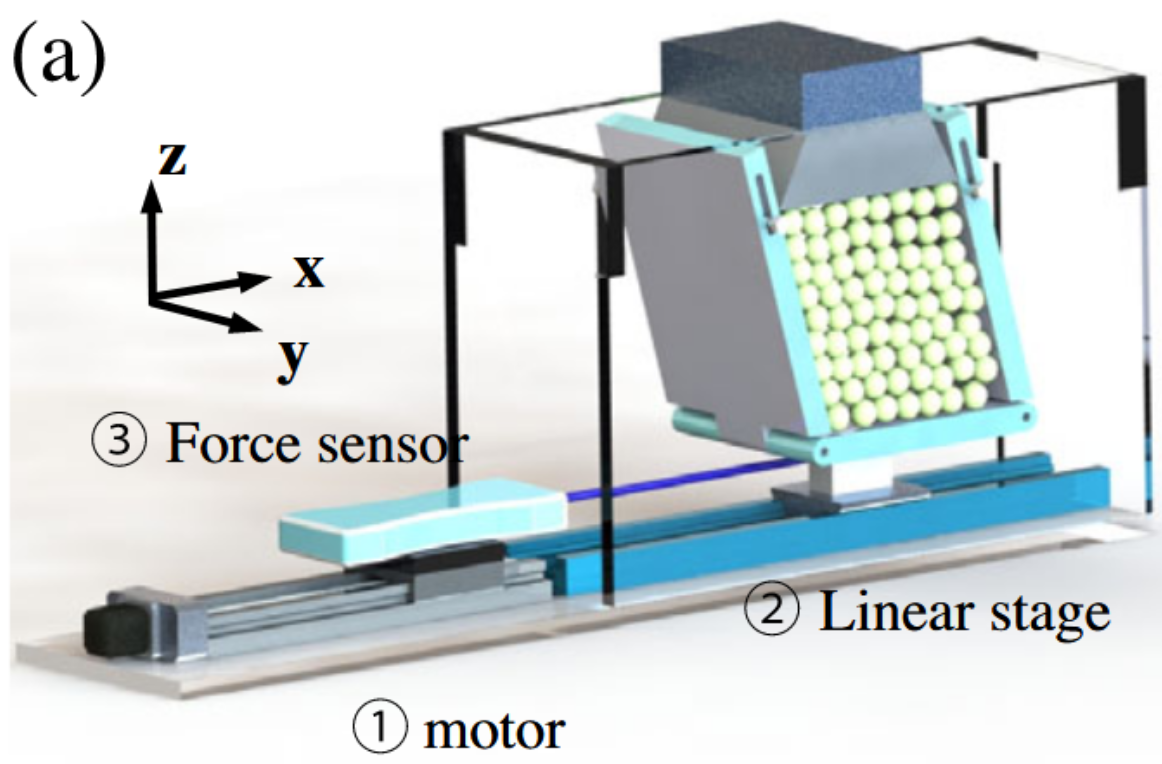
\includegraphics[height=3.5cm]{3_hloop_cycleshear_1.png}}
		\\
    \bisubcaptionbox{(a) 中颗粒介质的剪切应变 $\gamma$ 和体积分数 $\phi$、剪切应力 $F$ 的关系。}{Relationship between shear strain $\gamma$ and volume fraction $\phi$, and shear stress $F$ in granular media in (a).}
    [7cm]{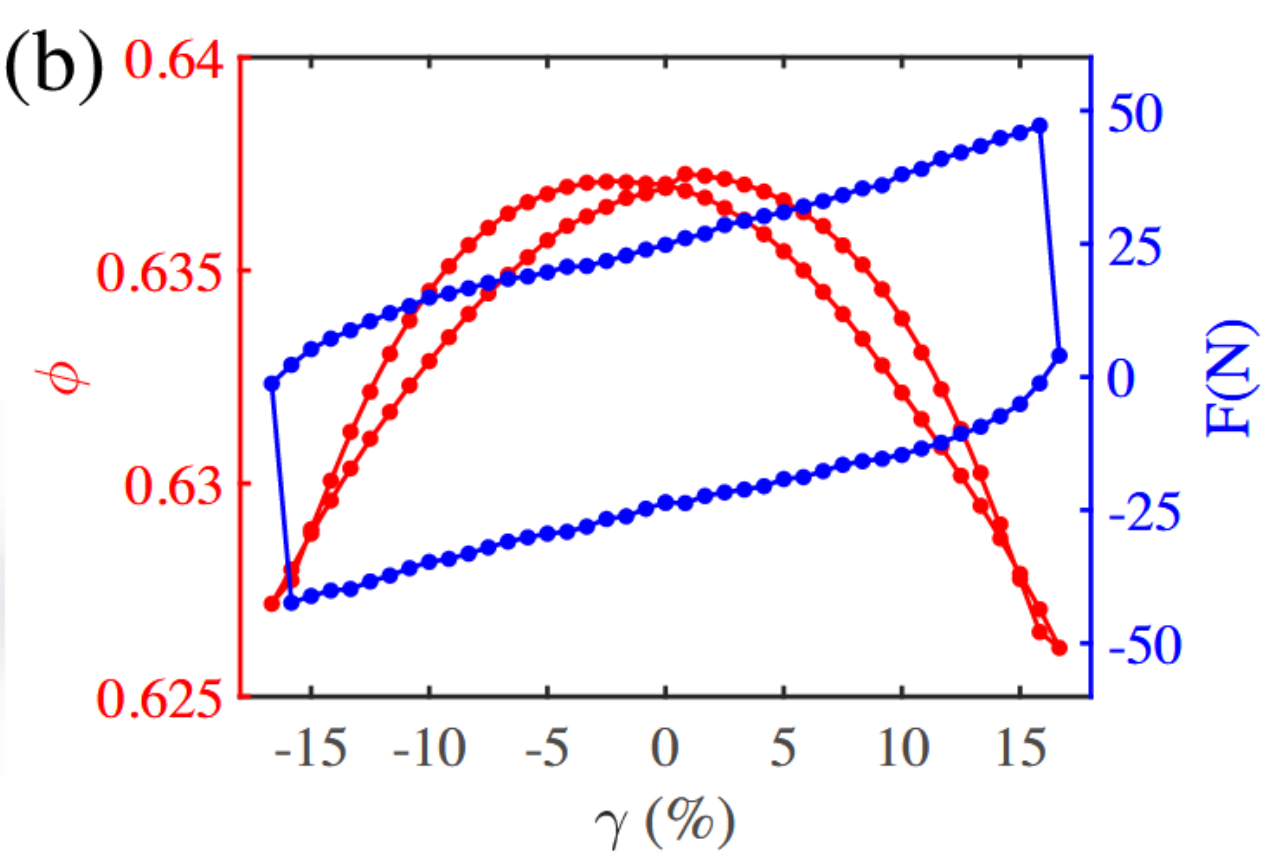
\includegraphics[height=3.5cm]{3_hloop_cycleshear_2.png}}
	\end{minipage}
	\begin{minipage}[!hbtp]{0.48\columnwidth}
		\centering
    \bisubcaptionbox{Xiaoping Jia 循环剪切实验中归一化剪切应力 $T$、剪切波(S)声速与剪切位移的演化关系。}{Evolution of normalized shear stress $T$, shear wave (S) velocity with shear displacement in Xiaoping Jia's cyclic shear experiment.}
    [7cm]{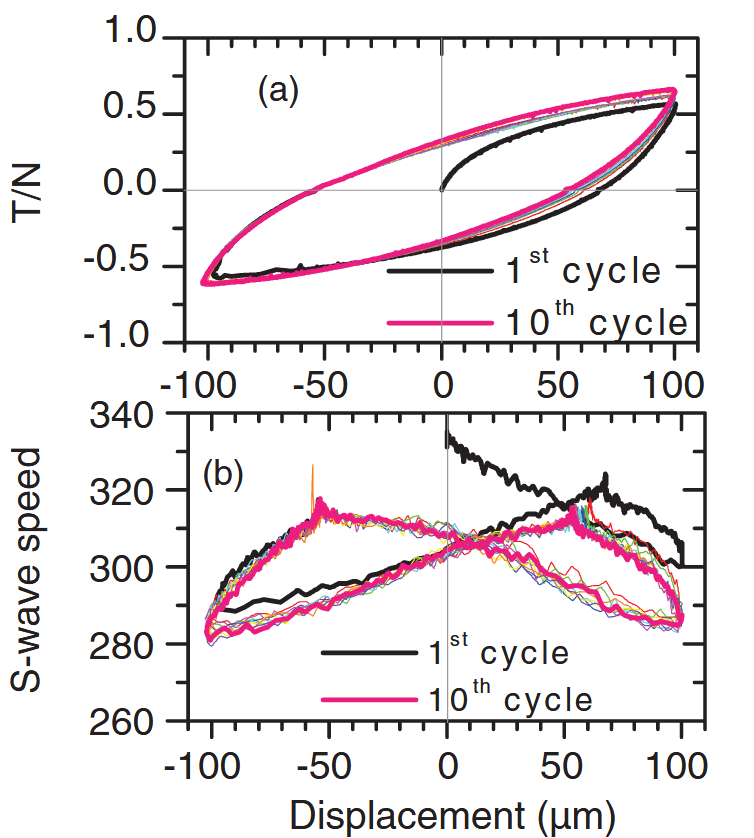
\includegraphics[height=7.5cm]{3_hloop_shearband.png}}
	\end{minipage}
	\bicaption{Yi Xing 与 Xiaoping Jia 在各自的循环剪切装置中都观察到了颗粒介质出现的滞回现象}{Hysteresis loops in granular media observed by Yi Xing and Xiaoping Jia in their respective cyclic shear apparatus.}\label{fig:hysteresis_loops}
\end{figure}

对于颗粒间的接触力同样存在着滞回现象。我们将切向振幅视为弹性响应分量(Elastic,E)和耗散响应分量(Hysteretic,H)的线性叠加,即

\begin{equation}
  u_{t}(f_{t}) = u_{t}^{E}(f_{t}) + su_{t}^{H}(f_{t}),\quad s = \begin{cases}
    1, & f_{t} \text{ increases},\\
    -1, & f_{t} \text{ decreases}.
  \end{cases}
\end{equation}

其中 $s$ 是一个与应力过程有关的符号函数。在切向应力最大幅值 $f_{t}^{*}$ 远小于颗粒间的静摩擦阈值 $\mu f_{0}$ 时,通过 Mindlin 接触可以推导出两种响应振幅的近似表达式:

\begin{align}
  u_{t}^{E}(f_{t}) &\approx \frac{2}{3}u_{0}\left(1 + \frac{f_{t}^{*}}{6\mu f_{0}}\right)\left(\frac{f_{t}}{\mu f_{0}}\right),\label{eq:elastic_amplitude}\\
  u_{t}^{H}(f_{t}) &\approx \frac{1}{18}u_{0}\left[\left(\frac{f_{t}}{\mu f_{0}}\right)^{2} - \left(\frac{f_{t}^{*}}{\mu f_{0}}\right)^{2}\right].
\end{align}

对于式~\eqref{eq:elastic_amplitude} 进行反求导,即可得到切向接触的刚度系数:

\begin{equation}
  D_{t}^{*} = \frac{\mathrm{d}f_{t}}{\mathrm{d}u_{t}^{E}} \approx D_{t}\left(1 - \frac{f_{t}^{*}}{6\mu f_{0}}\right)
\end{equation}

因此可以推导出声速的相对变化量表达式为

\begin{align}
  \frac{\Delta V}{V}\sim \frac{\Delta D_{t}}{D_{t}} &\approx -\frac{f_{t}^{*}}{6\mu f_{0}} \sim -ku_{t}^{*},\\
  k &= \frac{2G_{g}a}{3(2-\nu_{g})\mu f_{0}}\label{eq:friction}
\end{align}

其中 $G_{g}$、$\nu_{g}$ 是颗粒材料的剪切模量和泊松比。由此我们得出了两种可能的弹性软化机制。

\subsubsection{实验验证}

如果使用式~\eqref{eq:plane_wave} 来近似声信号在颗粒介质中的传播,我们可以使用类似于推导式~\eqref{eq:phase_velocity} 的方法得出衰减系数 $\alpha$ 的表达式:

\begin{equation}
  \alpha = \frac{1}{x_{2}-x_{1}}\ln{\left(\frac{S_{1}}{S_{2}}\right)}
\end{equation}

其中 $S_{1}$ 和 $S_{2}$ 分别是在 $x_{1}$ 和 $x_{2}$ 所采集信号在时域上的最大值(即去除含时系数)。但是在前面求解相速度的实验与讨论中我们已经知道,试图使用仅仅两道信号就对颗粒介质做出完整表述是几乎不可能的,需要进行系综平均以去除偶然性。因此在真正实验中,我们将使用类似于时差法测量声速的方法来测量衰减系数,即拟合声信号振幅的对数 $A$ 和传播距离/颗粒介质厚度 $L$ 的线性关系,其中斜率为 $-\alpha = \mathrm{d}[\ln{A}]/\mathrm{d}[L]$。

我们分别在应力为 9 \unit{\kilo\pascal} 和 \unit{\kilo\pascal} 的条件下,分别使用间歇激励和连续激励协议来对颗粒介质发射声信号,同时计算声速变化量、相似性参数与激励过程之间的关系。